
\chapter{Analysis of deep neural networks for predicting DNA methylation}

\ifpdf
    \graphicspath{{Chapter5/Figs/Raster/}{Chapter5/Figs/PDF/}{Chapter5/Figs/}}
\else
    \graphicspath{{Chapter5/Figs/Vector/}{Chapter5/Figs/}}
\fi

\begin{figure}[htbp!]
\centering
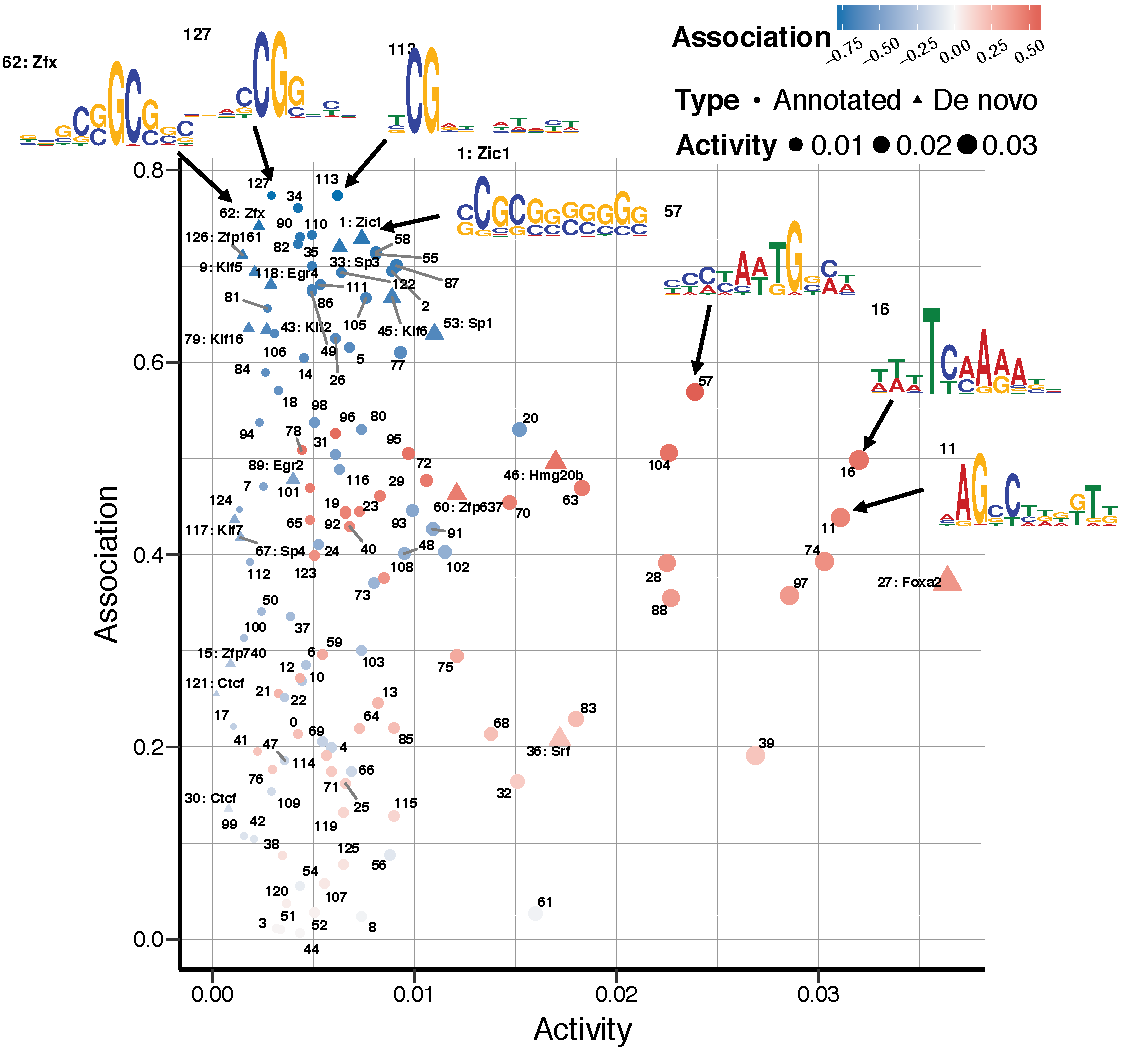
\includegraphics[width=0.8\textwidth]{motifs_imp}
\caption[Importance of the DNA sequence motifs learned by DeepCpG.]{Importance of the DNA sequence motifs learned by DeepCpG. Average motif activity on the x-axis vs. the absolute estimated motif effect on methylation (association) on the y-axis. Marker size and colour correspond to the activity of motifs, and their association with methylation states, respectively. Triangles denote annotated motifs (matched to motif in CIS-BP or UniPROPE database; $\FDR<0.05$); circles denote de novo motifs.}
\label{fig:dcpg_motifs_imp}
\end{figure}

\begin{figure}[htbp!]
\centering
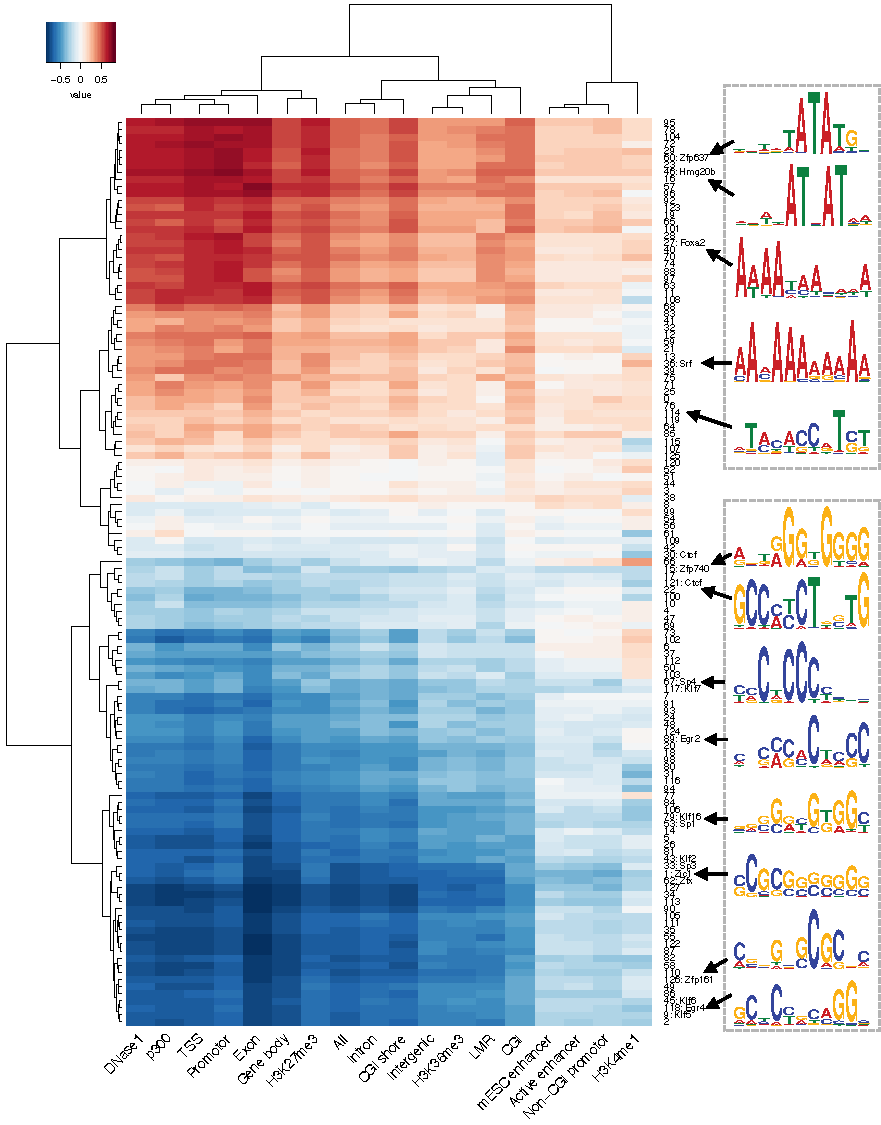
\includegraphics[width=1.0\textwidth]{motifs_cor}
\caption[Effect of DNA sequence motifs on methylation.]{Effect of DNA sequence motifs on methylation. Effect of discovered motifs on CpG methylation in different genomic contexts on test chromosomes, quantified by Pearson correlation between motif activities and predicted methylation level. Motifs cluster into CG-rich, methylation-decreasing motifs, and AT-rich methylation-increasing motifs.}
\label{fig:dcpg_motifs_cor}
\end{figure}

\begin{figure}[htbp!]
\centering
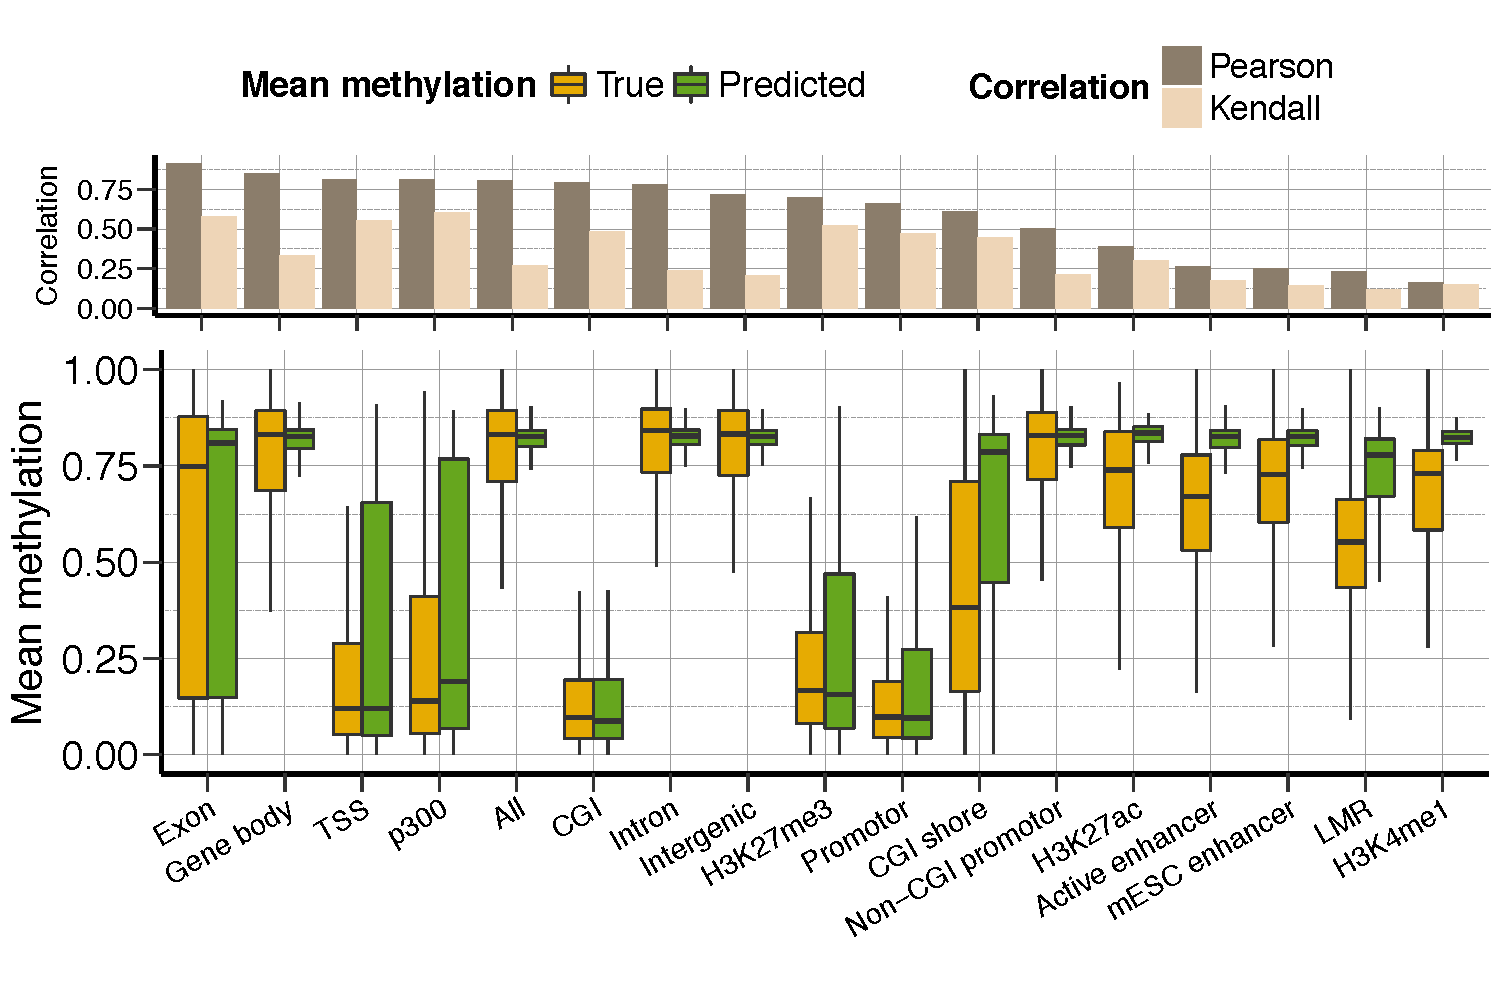
\includegraphics[width=1.0\textwidth]{var_mean}
\caption[Prediction performance of mean methylation levels.]{Performance of DeepCpG DNA module to predict mean methylation levels. Boxplot represent predicted (green) and the observed (orange) mean methylation levels in 3~kbp windows centred on individual CpG sites for different genomic contexts on held out test chromosomes. Barplot represent Pearson and Kendall correlation coefficients.}
\label{fig:dcpg_var_mean}
\end{figure}

\begin{figure}[htbp!]
\centering
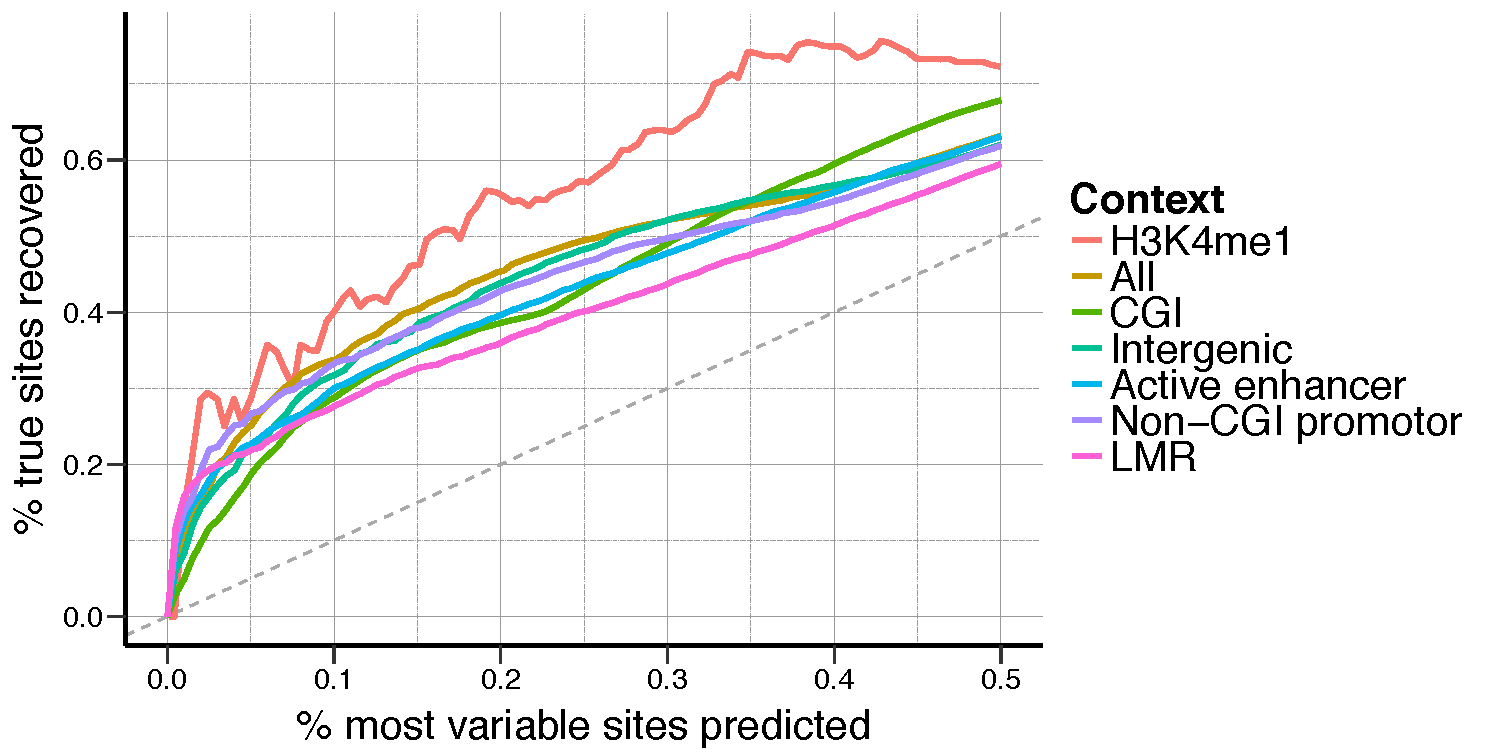
\includegraphics[width=0.9\textwidth]{var_rank}
\caption[Sensitivity of discovering highly-variable CpG sites.]{Sensitivity of discovering highly-variable CpG sites. Sensitivity of discovering most variable sites for different thresholds and genomic contexts on test chromosomes. Individual CpG sites were ranked by the empirical variance estimated in 3~kbp windows centred on the CpG sites, or the variance predicted by DeepCpG, and the overlap computed for the fraction of most variables sites shown on the x-axis. The dashed line indicates the performance of a random ranking.}
\label{fig:dcpg_var_rank}
\end{figure}

\begin{figure}[htbp!]
\centering
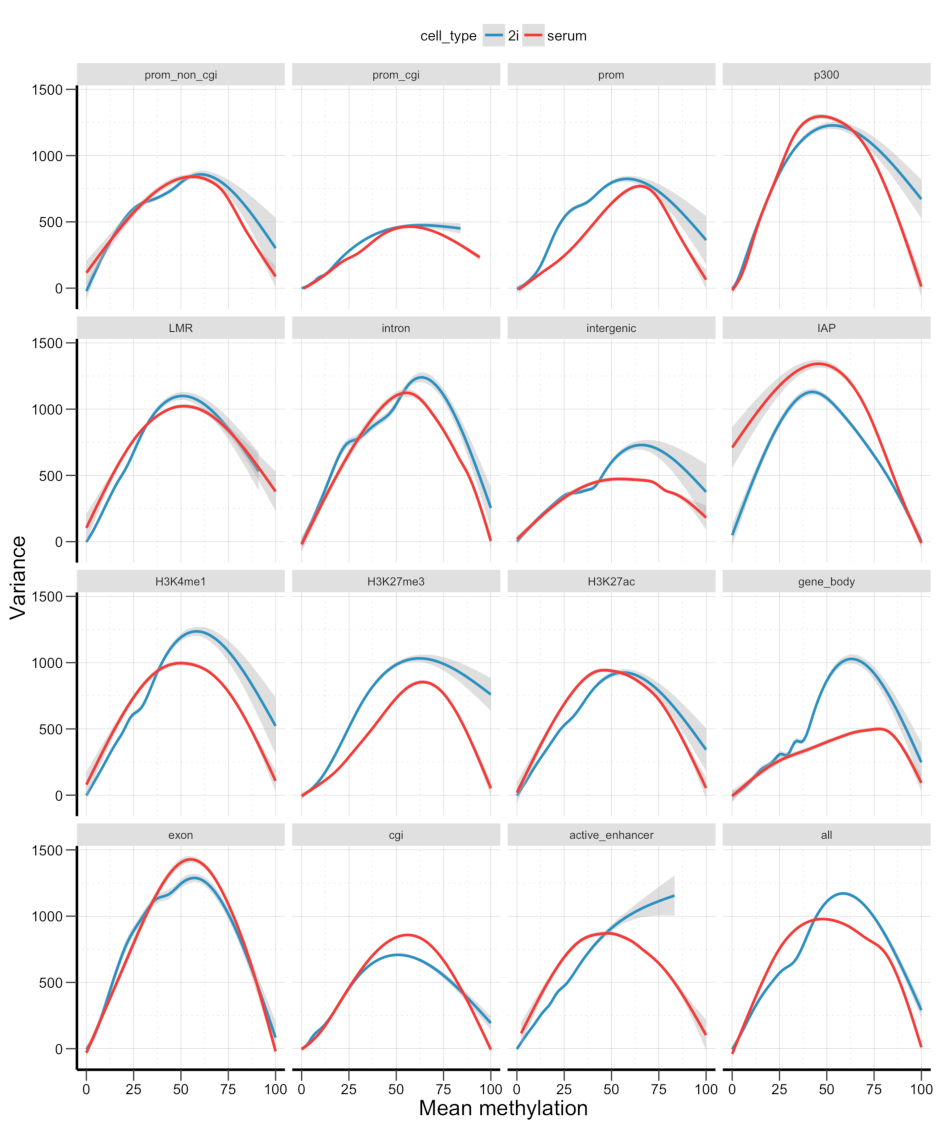
\includegraphics[width=1.0\textwidth]{var_couple}
\caption[Dependency between mean methylation levels and cell-to-cell variance.]{Dependency between mean methylation levels and cell-to-cell variance. Smoothed regression fit between mean methylation levels (x-axis) verus cell-to-cell variance (y-axis), for 2i and serum cells in different genomic contexts. Cell-to-cell variance is linked to the mean methylation level, and highest for an intermediate methylation level of 50\%.}
\label{fig:dcpg_var_couple}
\end{figure}

\begin{figure}[htbp!]
\centering
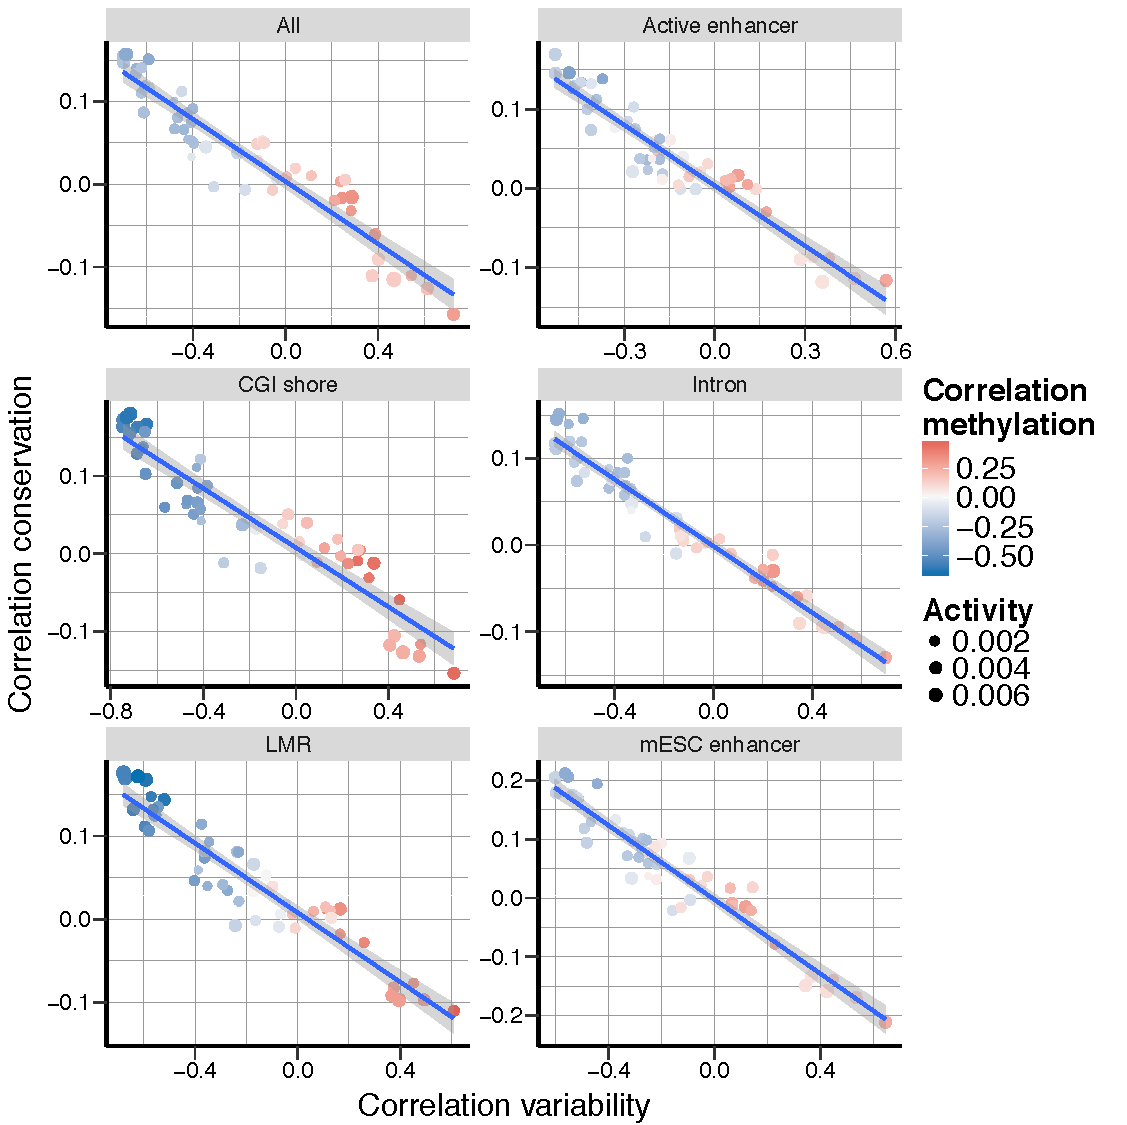
\includegraphics[width=1.0\textwidth]{var_cons}
\caption[Linkage between motif correlation with sequence conservation and cell-to-cell variability.]{Linkage between motif correlation with sequence conservation and cell-to-cell variability. Correlation of motif activities with cell-to-cell variability (x-axis), and DNA conservation (y-axis). Variability increasing motifs are most active in non-conserved regions. Individual dots correspond to motifs with their mean activity represented by the size, and influence on CpG methylation by colour.}
\label{fig:dcpg_var_cons}
\end{figure}

\begin{figure}[htbp!]
\centering
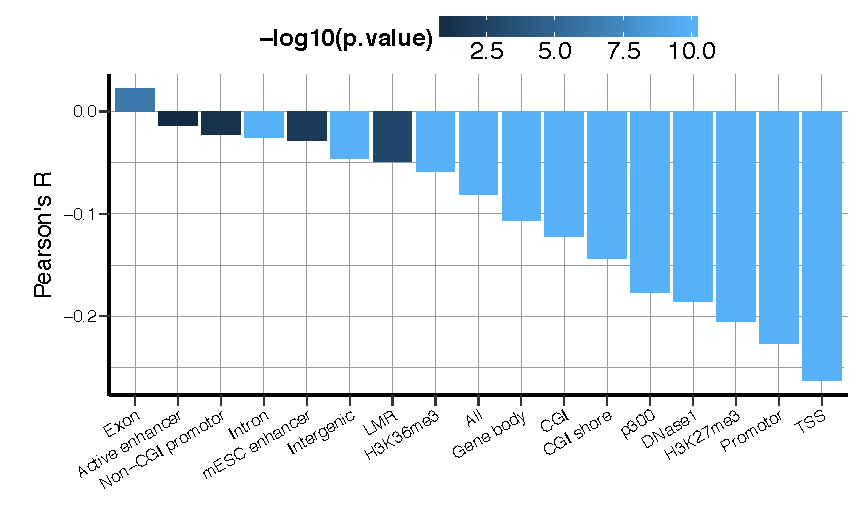
\includegraphics[width=1.0\textwidth]{mut_cons}
\caption[Correlation between estimated mutation effects and DNA sequence conservation.]{Correlation between estimated mutation effects and DNA sequence conservation. Correlation between the estimated effect of single-nucleotide mutations and PhastCons conservation score for alternative contexts on test chromosomes. Estimated effects are significantly anti-correlated overall (`All', $P<1.0\times10^{-15}$) in CpG dense regions.}
\label{fig:dcpg_mut_cons}
\end{figure}
